\documentclass{standalone}
\usepackage{pgfplots}
\pgfplotsset{compat=1.18}
\usepgfplotslibrary{fillbetween}

\begin{document}
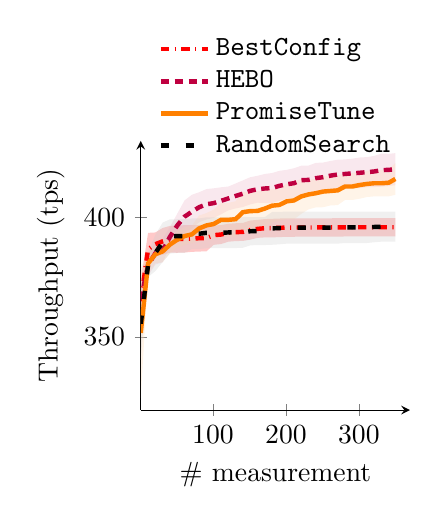
\begin{tikzpicture}
    \begin{axis}[
      axis x line  = bottom,
      axis y line  = left,
      width=5cm, height=5cm, 
      xlabel={\# measurement},
      ylabel={Throughput (tps)},
      xmin=1.0000, xmax=370.0000,
      ymin=319.2998, ymax=432.0564,
      legend cell align=left,
      legend columns=1,
      legend style={
        draw=none, fill=none,
        at={(0.98,0.9)}, anchor=south east,
        legend cell align=left
      }
    ]


\addplot[
    red,
    dashdotted,
    ultra thick, forget plot
] coordinates {
(1.0000, 364.8670) (11.0000, 386.6799) (21.0000, 388.7840) (31.0000, 389.9738) (41.0000, 390.8321) (51.0000, 390.9315) (61.0000, 391.0207) (71.0000, 391.1581) (81.0000, 391.2815) (91.0000, 391.3649) (101.0000, 392.5626) (111.0000, 392.8347) (121.0000, 393.5867) (131.0000, 393.8300) (141.0000, 393.9399) (151.0000, 394.6979) (161.0000, 395.2030) (171.0000, 395.4727) (181.0000, 395.5313) (191.0000, 395.6528) (201.0000, 395.7365) (211.0000, 395.7555) (221.0000, 395.7929) (231.0000, 395.7929) (241.0000, 395.7946) (251.0000, 395.8143) (261.0000, 395.8143) (271.0000, 395.8407) (281.0000, 395.8511) (291.0000, 395.8841) (301.0000, 395.8841) (311.0000, 395.8841) (321.0000, 395.8869) (331.0000, 395.8869) (341.0000, 395.8869) (350.0000, 395.8869)
}; 
\addplot[
name path=upper0,
draw=none, forget plot
] coordinates {
(1.0000, 373.4632) (11.0000, 393.5293) (21.0000, 393.7059) (31.0000, 395.5769) (41.0000, 396.4375) (51.0000, 396.6644) (61.0000, 396.7431) (71.0000, 396.7377) (81.0000, 396.8534) (91.0000, 396.9478) (101.0000, 396.5945) (111.0000, 396.8254) (121.0000, 397.3360) (131.0000, 397.5632) (141.0000, 397.7230) (151.0000, 398.7017) (161.0000, 398.9766) (171.0000, 399.3016) (181.0000, 399.4235) (191.0000, 399.5461) (201.0000, 399.6041) (211.0000, 399.6111) (221.0000, 399.6287) (231.0000, 399.6287) (241.0000, 399.6286) (251.0000, 399.6498) (261.0000, 399.6498) (271.0000, 399.6796) (281.0000, 399.6879) (291.0000, 399.7281) (301.0000, 399.7281) (311.0000, 399.7281) (321.0000, 399.7266) (331.0000, 399.7266) (341.0000, 399.7266) (350.0000, 399.7266)
}; 

\addplot[
name path=lower0,
draw=none, forget plot
] coordinates {
(1.0000, 356.2707) (11.0000, 379.8305) (21.0000, 383.8621) (31.0000, 384.3708) (41.0000, 385.2267) (51.0000, 385.1985) (61.0000, 385.2982) (71.0000, 385.5786) (81.0000, 385.7097) (91.0000, 385.7819) (101.0000, 388.5306) (111.0000, 388.8440) (121.0000, 389.8374) (131.0000, 390.0969) (141.0000, 390.1568) (151.0000, 390.6941) (161.0000, 391.4293) (171.0000, 391.6438) (181.0000, 391.6391) (191.0000, 391.7595) (201.0000, 391.8689) (211.0000, 391.8999) (221.0000, 391.9571) (231.0000, 391.9571) (241.0000, 391.9605) (251.0000, 391.9788) (261.0000, 391.9788) (271.0000, 392.0019) (281.0000, 392.0142) (291.0000, 392.0402) (301.0000, 392.0402) (311.0000, 392.0402) (321.0000, 392.0472) (331.0000, 392.0472) (341.0000, 392.0472) (350.0000, 392.0472)
}; 

% ========= file shading =========
\addplot[
    red!70,
    fill opacity=0.30, forget plot
] fill between[
    of=upper0 and lower0,
];


\addplot[
    purple,
    densely dashed,
    ultra thick, forget plot
] coordinates {
(1.0000, 365.5387) (11.0000, 379.9866) (21.0000, 384.9880) (31.0000, 386.0793) (41.0000, 391.9038) (51.0000, 396.6123) (61.0000, 400.3063) (71.0000, 402.3887) (81.0000, 404.2742) (91.0000, 405.5162) (101.0000, 405.9844) (111.0000, 406.9618) (121.0000, 407.9468) (131.0000, 408.9938) (141.0000, 409.9516) (151.0000, 411.1402) (161.0000, 411.8029) (171.0000, 412.1237) (181.0000, 412.3171) (191.0000, 413.2259) (201.0000, 413.8876) (211.0000, 414.3417) (221.0000, 415.6097) (231.0000, 415.7203) (241.0000, 416.4565) (251.0000, 416.8643) (261.0000, 417.5008) (271.0000, 417.9942) (281.0000, 418.2102) (291.0000, 418.4644) (301.0000, 418.6986) (311.0000, 418.9631) (321.0000, 419.2526) (331.0000, 419.8146) (341.0000, 419.9274) (350.0000, 420.2189)
}; 
\addplot[
name path=upper1,
draw=none, forget plot
] coordinates {
(1.0000, 377.1766) (11.0000, 384.5038) (21.0000, 389.6939) (31.0000, 390.9686) (41.0000, 395.9814) (51.0000, 401.5625) (61.0000, 407.1239) (71.0000, 409.4787) (81.0000, 410.5636) (91.0000, 411.8791) (101.0000, 412.2020) (111.0000, 412.6230) (121.0000, 412.9426) (131.0000, 414.2199) (141.0000, 415.5265) (151.0000, 416.8355) (161.0000, 417.4381) (171.0000, 418.2037) (181.0000, 418.6033) (191.0000, 419.5210) (201.0000, 419.9344) (211.0000, 420.6115) (221.0000, 421.6551) (231.0000, 421.7374) (241.0000, 422.8549) (251.0000, 422.9904) (261.0000, 423.6627) (271.0000, 424.1788) (281.0000, 424.2956) (291.0000, 424.6228) (301.0000, 425.0985) (311.0000, 425.2648) (321.0000, 425.7878) (331.0000, 426.7585) (341.0000, 426.6507) (350.0000, 426.9311)
}; 

\addplot[
name path=lower1,
draw=none, forget plot
] coordinates {
(1.0000, 353.9008) (11.0000, 375.4693) (21.0000, 380.2822) (31.0000, 381.1899) (41.0000, 387.8261) (51.0000, 391.6622) (61.0000, 393.4886) (71.0000, 395.2986) (81.0000, 397.9848) (91.0000, 399.1533) (101.0000, 399.7668) (111.0000, 401.3006) (121.0000, 402.9510) (131.0000, 403.7677) (141.0000, 404.3766) (151.0000, 405.4449) (161.0000, 406.1678) (171.0000, 406.0437) (181.0000, 406.0309) (191.0000, 406.9308) (201.0000, 407.8409) (211.0000, 408.0719) (221.0000, 409.5643) (231.0000, 409.7032) (241.0000, 410.0581) (251.0000, 410.7382) (261.0000, 411.3390) (271.0000, 411.8096) (281.0000, 412.1248) (291.0000, 412.3060) (301.0000, 412.2986) (311.0000, 412.6615) (321.0000, 412.7174) (331.0000, 412.8706) (341.0000, 413.2042) (350.0000, 413.5067)
}; 

% ========= file shading =========
\addplot[
    purple!30,
    fill opacity=0.30, forget plot
] fill between[
    of=upper1 and lower1,
];


\addplot[
    orange,
    solid,
    ultra thick, forget plot
] coordinates {
(1.0000, 351.6251) (11.0000, 380.7228) (21.0000, 384.5537) (31.0000, 385.7644) (41.0000, 388.6086) (51.0000, 390.6693) (61.0000, 392.2128) (71.0000, 392.8956) (81.0000, 395.3995) (91.0000, 396.6415) (101.0000, 397.2440) (111.0000, 398.9928) (121.0000, 398.9928) (131.0000, 399.2623) (141.0000, 402.1948) (151.0000, 402.6515) (161.0000, 402.7245) (171.0000, 403.7014) (181.0000, 404.9194) (191.0000, 405.2265) (201.0000, 406.7396) (211.0000, 407.1110) (221.0000, 408.7953) (231.0000, 409.6363) (241.0000, 410.1506) (251.0000, 410.8308) (261.0000, 411.0839) (271.0000, 411.3426) (281.0000, 412.9587) (291.0000, 412.9587) (301.0000, 413.5714) (311.0000, 414.0286) (321.0000, 414.3216) (331.0000, 414.3216) (341.0000, 414.5352) (350.0000, 416.1049)
}; 
\addplot[
name path=upper2,
draw=none, forget plot
] coordinates {
(1.0000, 378.8250) (11.0000, 385.0323) (21.0000, 388.2476) (31.0000, 390.3356) (41.0000, 392.1784) (51.0000, 394.1455) (61.0000, 396.0290) (71.0000, 396.5719) (81.0000, 400.8332) (91.0000, 401.8202) (101.0000, 403.2677) (111.0000, 406.0766) (121.0000, 406.0766) (131.0000, 406.7770) (141.0000, 410.6879) (151.0000, 410.8308) (161.0000, 410.8827) (171.0000, 411.3193) (181.0000, 411.9361) (191.0000, 411.8118) (201.0000, 414.1862) (211.0000, 415.0515) (221.0000, 416.0976) (231.0000, 415.8806) (241.0000, 416.0873) (251.0000, 417.3921) (261.0000, 417.1382) (271.0000, 417.5382) (281.0000, 418.6007) (291.0000, 418.6007) (301.0000, 419.3006) (311.0000, 419.5117) (321.0000, 419.8237) (331.0000, 419.8237) (341.0000, 420.2313) (350.0000, 422.7402)
}; 

\addplot[
name path=lower2,
draw=none, forget plot
] coordinates {
(1.0000, 324.4251) (11.0000, 376.4132) (21.0000, 380.8599) (31.0000, 381.1932) (41.0000, 385.0388) (51.0000, 387.1931) (61.0000, 388.3965) (71.0000, 389.2193) (81.0000, 389.9658) (91.0000, 391.4627) (101.0000, 391.2203) (111.0000, 391.9089) (121.0000, 391.9089) (131.0000, 391.7477) (141.0000, 393.7017) (151.0000, 394.4722) (161.0000, 394.5663) (171.0000, 396.0835) (181.0000, 397.9027) (191.0000, 398.6413) (201.0000, 399.2931) (211.0000, 399.1706) (221.0000, 401.4930) (231.0000, 403.3920) (241.0000, 404.2140) (251.0000, 404.2694) (261.0000, 405.0295) (271.0000, 405.1469) (281.0000, 407.3168) (291.0000, 407.3168) (301.0000, 407.8423) (311.0000, 408.5456) (321.0000, 408.8195) (331.0000, 408.8195) (341.0000, 408.8390) (350.0000, 409.4696)
}; 

% ========= file shading =========
\addplot[
    orange!30,
    fill opacity=0.30, forget plot
] fill between[
    of=upper2 and lower2,
];


\addplot[
    black,
    loosely dashed,
    ultra thick, forget plot
] coordinates {
(1.0000, 355.4614) (11.0000, 380.0976) (21.0000, 385.1373) (31.0000, 389.5853) (41.0000, 392.0252) (51.0000, 392.1701) (61.0000, 392.1701) (71.0000, 393.1681) (81.0000, 393.1681) (91.0000, 393.5652) (101.0000, 393.5652) (111.0000, 393.5652) (121.0000, 393.7039) (131.0000, 393.7039) (141.0000, 393.7545) (151.0000, 394.2101) (161.0000, 394.2833) (171.0000, 394.2833) (181.0000, 395.4129) (191.0000, 395.5283) (201.0000, 395.7242) (211.0000, 395.7335) (221.0000, 395.7335) (231.0000, 395.7335) (241.0000, 395.7335) (251.0000, 395.7335) (261.0000, 395.7335) (271.0000, 395.7335) (281.0000, 395.8579) (291.0000, 395.8579) (301.0000, 395.8579) (311.0000, 395.8579) (321.0000, 396.0001) (331.0000, 396.1307) (341.0000, 396.1307) (350.0000, 396.1307)
}; 
\addplot[
name path=upper3,
draw=none, forget plot
] coordinates {
(1.0000, 369.9149) (11.0000, 385.1671) (21.0000, 392.7472) (31.0000, 397.8244) (41.0000, 399.1971) (51.0000, 399.2398) (61.0000, 399.2398) (71.0000, 399.5735) (81.0000, 399.5735) (91.0000, 400.0303) (101.0000, 400.0303) (111.0000, 400.0303) (121.0000, 400.2412) (131.0000, 400.2412) (141.0000, 400.2138) (151.0000, 400.1345) (161.0000, 400.1321) (171.0000, 400.1321) (181.0000, 402.2812) (191.0000, 402.3251) (201.0000, 402.4390) (211.0000, 402.4370) (221.0000, 402.4370) (231.0000, 402.4370) (241.0000, 402.4370) (251.0000, 402.4370) (261.0000, 402.4370) (271.0000, 402.4370) (281.0000, 402.4315) (291.0000, 402.4315) (301.0000, 402.4315) (311.0000, 402.4315) (321.0000, 402.4071) (331.0000, 402.4063) (341.0000, 402.4063) (350.0000, 402.4063)
}; 

\addplot[
name path=lower3,
draw=none, forget plot
] coordinates {
(1.0000, 341.0079) (11.0000, 375.0281) (21.0000, 377.5273) (31.0000, 381.3462) (41.0000, 384.8533) (51.0000, 385.1004) (61.0000, 385.1004) (71.0000, 386.7627) (81.0000, 386.7627) (91.0000, 387.1000) (101.0000, 387.1000) (111.0000, 387.1000) (121.0000, 387.1666) (131.0000, 387.1666) (141.0000, 387.2952) (151.0000, 388.2856) (161.0000, 388.4344) (171.0000, 388.4344) (181.0000, 388.5447) (191.0000, 388.7314) (201.0000, 389.0095) (211.0000, 389.0301) (221.0000, 389.0301) (231.0000, 389.0301) (241.0000, 389.0301) (251.0000, 389.0301) (261.0000, 389.0301) (271.0000, 389.0301) (281.0000, 389.2843) (291.0000, 389.2843) (301.0000, 389.2843) (311.0000, 389.2843) (321.0000, 389.5931) (331.0000, 389.8552) (341.0000, 389.8552) (350.0000, 389.8552)
}; 

% ========= file shading =========
\addplot[
    black!20,
    fill opacity=0.30, forget plot
] fill between[
    of=upper3 and lower3,
];


\addlegendimage{red, dashdotted, ultra thick}
\addlegendentry{\texttt{BestConfig}}
\addlegendimage{purple, densely dashed, ultra thick}
\addlegendentry{\texttt{HEBO}}
\addlegendimage{orange, solid, ultra thick}
\addlegendentry{\texttt{PromiseTune}}
\addlegendimage{black, loosely dashed, ultra thick}
\addlegendentry{\texttt{RandomSearch}}

\end{axis}
\end{tikzpicture}
\end{document}
